All CC Protocols discussed thus-far provide retailers with a property of credit card payments known as \emph{linkability}:
    retailers are able to link purchases made using the same card, in order to build purchasing profiles on their customers.
Customer purchasing profiles are valuable to retailers, because they allow for more targeted and effective marketing, and can be sold to interested third parties.

However, these purchasing profiles can be unpleasant to the customer from a privacy standpoint:
  purchasing habits can reveal sensitive and personal information.
Furthermore, a customer cannot opt-out of this profiling except by avoiding the use of credit cards.

Recall that in the Insecure CC Protocol described in Chapter \ref{cha:insecure} (and in widespread use today),
  the card discloses its card number, expiration date, and iCVV to the point of sale with every purchase.
Therefore, a retailer can link purchases simply by comparing card numbers of these purchases.
Any credit card protocol which gives the retailer access to the card number is linkable by definition.

With this in mind, we consider how to provide credit card payments with the converse property: \emph{unlinkability}.
Informally, if credit card purchases are unlinkable, then retailers cannot use them to construct purchasing profiles efficiently.

While giving the retailer access to the card number is sufficient to undermine unlinkability, it is not necessary.
For example, consider the Externally Secure CC Protocol, presented in Chapter \ref{cha:external} and shown in Figure \ref{fig:external_ccp_recall} for convenience.
In this protocol, the credit card number is not disclosed, and all authentication data (contained within the value \emph{T}) is indistinguishable from random to the retailer.
However, the charge token contains a constant card identifier \emph{ID}, required by the bank in order to identify the customer for which \emph{T} must be verified.
No two credit cards have the same \emph{ID}, and \emph{ID} does not change, so the retailer can simply link purchases using \emph{ID} instead of the card number.
More generally, if the protocol includes a message received by the retailer from which the customer's identity can be inferred, then the protocol cannot provide unlinkability.

\begin{figure}[h!]
  \caption{Externally Secure CC Protocol}
  \centering
    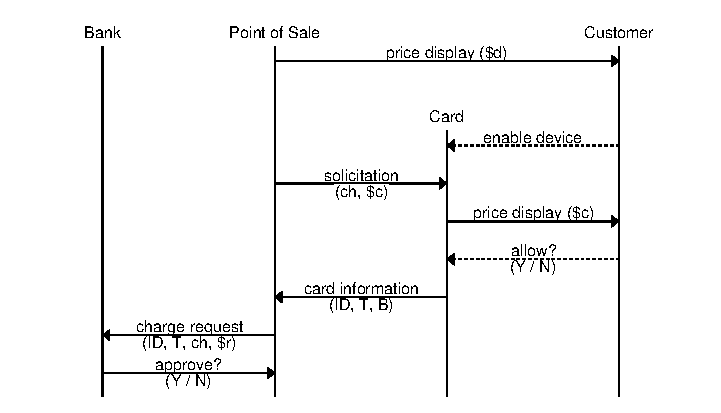
\includegraphics{img/secure_ccp.eps}
  \label{fig:external_ccp_recall}
\end{figure}


While we wish to conceal the customer's identity from the retailer, it must be disclosed to the bank in order for a charge to be processed.
As such, the problem reduces to one where we wish the contents of a message generated by a credit card (the message source)
  to be opaque to the point of sale (the carrier), but not to the bank (the final destination).
A natural approach to this problem is to use cryptography.

First let us consider symmetric cryptography, wherein the original sender (the credit card) and the final destination (the bank) share a secret key used for both encryption and decryption.
While symmetric cryptography can provide confidentiality of a message from the card to the bank, it cannot provide unlinkability.
This is because the message received by the bank must include some method for determining which of its customer's keys the bank should use to decrypt the message.
The retailer may then simply use this key identifier to link purchases.

Second, let us consider asymmetric (or ``public key'') cryptography,
  a system in which anybody (having access only to publicly available information) may encrypt a message that only the intended recipient may decrypt.
Indeed, it would not be difficult to construct a provably unlinkable payment protocol using asymmetric encryption:
a Card Information message may simply consist of the customer's credit card information, encrypted using the bank's public key.
The result is a Card Information message which is indistinguishable from random to the retailer.
The bank decrypts this message using its private key, reads the credit card information from the message body, and processes the payment.

Barring any other requirements, asymmetric cryptography provides sufficient primitives for constructing an unlinkable payment protocol.
However, asymmetric cryptography requires comparatively large (2048 bit) keys to be secure, and results in ciphertexts at least as long as the key.
For reasons to be discussed shortly in Section \ref{sec:goals-infrastructure}, we are limited to sending a single numeric 28-digit message to the point of sale.
As a result, using asymmetric cryptography in a secure manner is incompatible with our goals.

In conclusion, when constructing the Unlinkable CC Protocol, we need to define the Card Information message in such a way that it uniquely identifies the credit card to the bank,
  but where the entirety of the message is indistinguishable from random to the retailer,
  all while using at most 28 numeric digits.
